\chapter{Knowledge}
\label{cha:knowledgei}

\section{Prerequisites}
This section will introduce some important knowledges, including sigmoid function, Bayes Formula, Huffman code, etc.

\subsection{Sigmoid Function}
Sigmoid function is a common kind of active function, the definition is
$$ \sigma(x) = \frac{1}{1+e^{-x}}, $$
The domain is $(-\infty, \infty)$, the range is $(0,1)$. And Figure~\ref{fig:sigmoid} shows the sigmoid function.
\begin{figure}[!ht]
  \centering
	\fbox{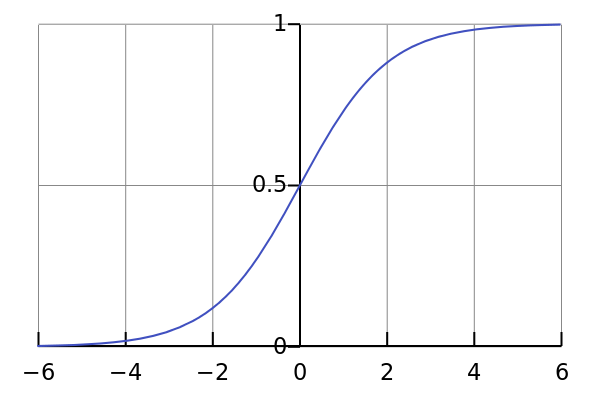
\includegraphics[width=0.5\textwidth]{sigmoid} }
	\caption{Sigmoid Function}
	\label{fig:sigmoid}
\end{figure}

Sigmoid function has the \textbf{derivative function} as following:
$$ \sigma^\prime(x) = \sigma(x)[1-\sigma(x)], $$
Thus, the \textbf{derivative functions} of $\mathrm{log}\sigma(x)$ and $\mathrm{log}(1-\sigma(x))$ are respectively
\begin{equation} 
[\mathrm{log}\sigma(x)]^\prime = 1-\sigma(x), \ [\mathrm{log}(1-\sigma(x))]^\prime = -\sigma(x), 
\end{equation}
Equation (2.1) will be used later in derivations.

\subsection{Logistic Regression}
Binary classification is a very common task, for example, if an email is spam, if a customer is a potential customer, if a online transaction fraud, etc. Let ${\{(\mathbf{x}_i,y_i)\}}^m_{i=1}$ be the sample data of a binary classification problem, where $\mathbf{x}_i \in \mathbb{R}^n$, $y_i \in \{0,1\}$, when $y_i = 1$ the corresponding sample is $\mathbf{positive}$, when $y_i = 0$ the corresponding sample is $\mathbf{negative}$.

As for some sample data $\mathbf{x} = (x_1,x_2,\cdots,x_n)^T$, the hypothesis function can be written as
$$h_\theta(\mathbf{x}) = \sigma(\theta_0+\theta_1 x_1+\theta_2 x_2+\cdots+\theta_n x_n),$$
where $\theta = (\theta_0,\theta_1,\cdots,\theta_n)^T$ is undetermined parameters. To simplify the formula, one can introduce $x_0 = 1$, and then $\mathbf{x}$ is extended to $(x_0,x_1,x_2,\cdots,x_n)^T$. Without confusing one can also record it as $\mathbf{x}$. Thus, $h_\theta$ can be simplified as 
$$h_\theta(\mathbf{x}) = \sigma(\theta^T \mathbf{x}) = \frac{1}{1+e^{-\theta^T \mathbf{x}}}.$$

Let threshold $T = 0.5$, then the discriminant formula for binary classification is
$$y(\mathbf{x})=
\begin{cases}
1,& h_\theta(\mathbf{x})\geq 0.5;\\
0,& h_\theta(\mathbf{x})\le 0.5.
\end{cases}$$

How to calculate $\theta$ ? A common method is, firstly one defines a form of the \textbf{overall loss function} as following
$$ J(\theta) = \frac{1}{m}\sum^m_{i=1}cost(\mathbf{x}_i,y_i),$$
and then one optimizes the overall loss function to obtain the optimal parameters $\theta^*$.

In practice, the loss function of a single sample $cost(\mathbf{x}_i,y_i)$ is often taken as the \textbf{log-likelihood function}
$$cost(\mathbf{x}_i,y_i)=
\begin{cases}
-\mathrm{log}(h_\theta(\mathbf{x}_i)),& y_i=1;\\
-\mathrm{log}(1-h_\theta(\mathbf{x}_i)),& y_i=0.
\end{cases}$$
Note that the above formula is a piecewise function, which can also be written in its overall expression as following
$$cost(\mathbf{x}_i,y_i) = -y_i\cdot\mathrm{log}(h_\theta(\mathbf{x}_i))-(1-y_i)\cdot\mathrm{log}(1-h_\theta(\mathbf{x}_i)).$$

\subsection{Bayes Formula}
Bayesian formula is put forward by the British mathematician Thomas Bayes, used to describe the relationship between two conditional probabilities. Let $P(A)$ and $P(B)$ respectively be the probability of event A and the probability of event B, $P(A|B)$ be the probability of the event A when event B occurs, and $P(A,B)$ be the probability of event A and B occurring simultaneously, so we have
$$P(A|B)=\frac{P(A,B)}{P(B)}, P(B|A)=\frac{P(A,B)}{P(A)}, $$
further, we can get
$$P(A|B)=P(A)\frac{P(B|A)}{P(B)},$$
the above formula is the \textbf{Bayes formula}.

\subsection{Huffman Coding}

\subsubsection{Huffman Tree}
In computer science, \textbf{tree} is a kind of nonlinear data structure, from which data elements (called \textbf{nodes} in the tree) organized in branch. The collection of several disjoint trees is called \textbf{forest}. The following concepts are some common concepts about tree.
\begin{itemize}
\item \textbf{Path} and \textbf{Path Length}\\
In a tree, a path is a road from any node to its direct or indirect child. The number of branches is called path length of the path. If the layer of the root node is $1$, the path length from the root node to nodes in the layer $L$ is $L-1$.
\item \textbf{Weight of a Node} and \textbf{Path Length with Weight of a Node}\\
Giving a node in a tree some value (non-negative), this value is called the weight of the node. The path length with weight of a node is the product of the path length from the root node to this node and the weight of this node.
\item \textbf{Path Length with Weight of a Tree}\\
The path length with weight of a tree is the sum of path length with weight of every leaf node.
\end{itemize}

A \textbf{Binary tree} is an ordered tree in which each node has at most two sub-trees. Two sub-trees are usually called \lq\lq Left Sub-Tree\rq\rq\ and \lq\lq Right Sub-Tree\rq\rq , the \lq\lq ordered\rq\rq\ means the order of left and right can not be reversed for two sub-trees.

Giving $n$ weights as weights of $n$ leaf nodes, one can build a binary tree. From all built trees, the one with the smallest path length with weight is called \textbf{Optimal Binary Tree}, which is also named \textbf{Huffman Tree}.
\subsubsection{Huffman Tree Construction}
Giving $n$ weights $\{w_1,w_2,\cdots,w_n\}$ as $n$ leaf nodes, one can build a Huffman tree as the following algorithm.
\paragraph{Algorithm 2.1}(\emph{Huffman Tree} Construction)
\begin{enumerate}
\item Consider $\{w_1,w_2,\cdots,w_n\}$ as root weights of $n$ trees in a forest (each tree has only one node).
\item Select the two trees in the forest with the smallest root weight, and combine them to be a new tree. These two trees are the left and right sub-trees of the new tree, and the root weight of the new tree is the sum of root weights of its sub-trees.
\item Remove above two trees from the forest, and add the new tree into the forest.
\item Repeat Step 2 and Step 3, until there is only one tree in the forest. Such tree is the \emph{Huffman Tree}.
\end{enumerate}
\paragraph{Example 2.1} Assuming in one news words \lq\lq I\rq\rq\ \lq\lq don't\rq\rq\ \lq\lq have\rq\rq\ \lq\lq putting\rq\rq\ \lq\lq money\rq\rq\ \lq\lq in\rq\rq\ \lq\lq my\rq\rq\ \lq\lq bank\rq\rq\ \lq\lq account\rq\rq\ appear respectively 5, 7, 20, 14, 6, 3, 16, 5, 10 times. One can build an \emph{Huffman Tree} with these 9 words as leaf nodes, and use word frequencies to be the weights of nodes.

Figure... shows the construction of the \emph{Huffman Tree}. From above, we can know that \textbf{the word with greater frequency is closer to the root node}. During the construction, new nodes after combination are marked blue. If there are $n$ leaf nodes, there will be $n-1$ new nodes in the built \emph{Huffman Tree}. In above example $n=6$, thus the number of new nodes is $5$. 

Note that, two sub binary trees is left and right, for a non-leaf node, it is its child nodes is two minutes.
\subsubsection{Huffman Coding}
In data communication, it is necessary to transfer the text into a binary string. One can use different permutations of 0,1 code to represent characters. For example, 


%--------------------------------------------------------------------------------------------------------------------------------%

\section{Background Knowledge}
\subsection{Statistical Language Model}
Nowadays, the Internet is developing very fast and generates a lot of text, image, voice, and video data every day. Natural language processing technology is necessary for processing these data and digging out valuable information. And the statistical language model is an very important part, which is widely used in speech recognition, machine translation, word segmentation, POS tagging and information retrieval. 
\paragraph{Example 2.2} In the speech recognition system, for a given speech segment \emph{Voice}, one needs to find a text segment \emph{Text} to make the probability $p(Text|Voice)$ the largest. Using \emph{Bayes} formula, we have
$$p(Text|Voice)=\frac{p(Voice|Text)\cdot p(Text)}{p(Voice)}$$
where $p(Voice|Text)$ is the \textbf{Acoustic Model}, and $p(Text)$ is the \textbf{Language Model}.

In short, statistical language model is a \textbf{Probability Model} to calculate the probability of an sentence, which is always built on a corpus. Assuming $W=w^T_1:=(w_1,w_2,\ldots,w_T)$ represents a sentence built by $T$ ordered words $w_1,w_2,\ldots,w_T$, and the joint probability of them is
$$p(W)=p(w^T_1)=p(w_1,w_2,\ldots,w_T)$$
the above is the probability of the sentence. Using \textbf{Bayes Formula}, the above formula can be decomposed as
\begin{equation}
p(w^T_1) = p(w_1)\cdot p(w_2|w_1)\cdot p(w_3|w^2_1)\ldots p(w_T|w^{T-1}_1),
\end{equation}
where the conditional probabilities $p(w_1),p(w_2|w_1),p(w_3|w^2_1),\ldots,p(w_T|w^{T-1}_1)$ are the \textbf{Language Model Parameters}. If all these parameters are calculated, giving a sentence $w^T_1$, one can get $p(w^T_1)$ quickly.

It seems very simple. But the implementation still have some trouble. For example, let's look at \textbf{the number of model parameters}. Considering a sentence with the length of $T$, we need to calculate $T$ parameters. Let's assume the size of dictionary $D$ (vocabulary) is $N$, considering any sentence with the size of $T$, there are theoretically $N^T$  possible sentences, and each sentence needs to be calculated T parameters, totally $TN^T$ parameters. Of course, the above is just a simple estimation and do not consider the arguments repeated, but the magnitude is still scary. In addition, storing these probabilities require a lot of memory.

So, how to calculate these parameters? There are some common methods such as n-gram model, decision tree, maximum entropy, maximum entropy Markov model, CRFs, neural networks and etc. This thesis discusses only n-gram model and neural network model. Firstly let's look at the n-gram model.
%--------------------------------------------------------------------------------------------------------------------------------%

\subsection{N-gram Model}
Considering the approximate calculation of $p(w_k|w^{k-1}_1) (k > 1)$. Using \emph{Bayes Formula}, we have
$$ p(w_k|w^{k-1}_1)=\frac{p(w_k|w^{k-1}_1)}{p(w^{k-1}_1)},$$
According to the Law of Large Numbers, when corpus is big enough, $p(w_k|w^{k-1}_1)$ can be approximately represented as
\begin{equation}
p(w_k|w^{k-1}_1)\approx \frac{count(w^k_1)}{count(w^{k-1}_1)}
\end{equation}
where $count(w^k_1)$ and $count(w^{k-1}_1)$ represent respectively the number of occurrences of word series $w^k_1$ and $w^{k-1}_1$. You can imagine, when $k$ is very large, the calculation of $count(w^k_1)$ and $count(w^{k-1}_1)$ really costs time. 
From the formula (), we can see: the probability of a word is related with all words before it. What if assuming the probability of a word is only related with its previously fixed number of words? Such is the main idea of \textbf{n-gram model}, which makes a $n-1$ ordered \textbf{Markov Assumption}, considering the occurrence probability of a word is only related with its previous $n-1$ words, that is 
$$p(w_k|w^{k-1}_1)\approx p(w_k|w^{k-1}_{k-n+1}),$$
thus,() becomes 
$$p(w_k|w^{k-1}_1)\approx \frac{count(w^k_{k-n+1}}{count(w^{k-1}_{k-n+1})}.$$
Making $n=2$ as the example, we have
$$p(w_k|w^{k-1}_1)\approx \frac{count(w_{k-1},w_k)}{count(w_{k-1})}.$$
The simplization makes the counting easier and the number of total parameters smaller.

So, how large is suitable for the parameter $n$ in n-gram model? Generally,  the election of $n$ depends on both the computational complexity and the model effect. 

As for \textbf{Computational Complexity}, the above shows the changing of  the number of model parameters when n becoming lager gradually, assuming the size of dictionary is $N = 200000$. Actually, the magnitude of the model parameters is the exponential function of $N$ ($O(N^n)$), obviously $n$ can not be too big. In the real application, $n=3$ is used the most.

As for \textbf{Model Effect}, theoretically, the larger $n$, the better effect. Nowadays, the big data from internet and the improvement machine performance make it possible to calculate more ordered language model (i.e. $n > 10$). But one thing needs to be noticed that when $n$ is big enough, the improvement of model effect will become small. For example, when $n$ becomes 2 from 1, and becomes 3 from 2, the improvement of model effect is obvious. However, when n becomes 4 from 3, the improvement of model effect if not so obvious. Actually, here refers to the reliability and distinguishability. If the parameters are more, the distinguishability will be better, but reliability is reduced because of fewer samples of each parameter. Thus, we need to compromise between reliability and distinguishability. 

In addition, there is a important part called smoothing in the model. Back to (), considering
\begin{enumerate}
\item If $count(w^k_{k-n+1})=0$,can we consider that $p(w_k|w^{k-1}_1) = 0$?
\item If $count(w^k_{k-n+1})=count(w^{k-1}_{k-n+1})$,can we consider that $p(w_k|w^{k-1}_1)=1$?
\end{enumerate}
Obviously not. But it is a very important question, no matter how big your corpus is. Smoothing is to deal with such problem. We won't discuss it here.

In conclusion, n-gram model is such kind of model, whose main working is to count the word seire in the corpus and then do smoothing. Storing the probabilities after calculation, if we need the probability of a sentence, we only need to find out the related probability parameters and then combine them.

In fact, there is a general method in machine learning: Build an object function after modelling a problem, and then optimize such object function, so that you can get a set of optimal parameters. Finally use corresponding model of these optimal parameters to do prediction. 

As for the statistical language model, using \textbf{Maximum Likelihood}, we can set the object function as 
$$\prod_{w\in C}p(w|Context(w)).$$
where $C$ represents the corpus, $Context(w)$ represents the context of  $w$, that is the set of words surrounding $w$. When $Context(w)$ is empty, we can set $p(w|Context(w))=p(w)$. Especially, as for the n-gram model, we have $Context(w_i)=w^{i-1}_{i-n+1}.$
\paragraph{Note 3.1} The difference between the corpus $C$ and the dictionary $D$:  The dictionary $D$ is extracted from the corpus $C$, without repeated words; while the corpus $C$ represents all text content, including repeated words.\\

Of course,  in the real application, the maximum log likelihood is used often, that is, set the object function as 
$$L=\sum_{w\in C} \mathrm{log}\ p(w|Context(w)),$$
And then optimise this function. 

From (), we can consider the probability $p(w|Context(w))$ as the function of $w$ and $Context(w)$
$$p(w|Context(w))=F(w,Context(w),\theta),$$
where $\theta$ is the \textbf{undetermined parameters set}. Thus, after optimization, we get $\theta^*$, and any probability $p(w|Context(w))$ can be calculated by the function $F(w,Context(w),\theta^*)$. Comparison with n-gram model, such method does not need to store all probabilities advance, instead one can obtain the function value by calculating directly. Also, if we choose proper model, the number of parameters in $\theta$ will be much smaller than one in the n-gram model.

Obviously, as for such method, the most important thing is \textbf{the building of function} \emph{\textbf{F}} . The next section will introduce a method using neural network to build $F$. 
%--------------------------------------------------------------------------------------------------------------------------------%
\subsection{Neural Probabilistic Language Model}
This section will introduce a neural probabilistic language model from \textbf{Bengio}. Such model use a very important tool---\textbf{Word Vector}.
So what is the word vector? General speaking, for any word $w$ in the dictionary $D$, one can specify a fixed length of real-valued vector $v(w)\in \mathbb{R}^m$, $v(w)$ called the word vector of $w$, and $m$ is the length of word vector. A further understanding about the word vectors will be explained in the next section. 

Since it is a neural probabilistic language model, it is obvious to use an neural network. Figure 4 shows the structure of the neural network, it include 4 layers: \textbf{Input} layer, \textbf{Projection} layer, \textbf{Hidden} layer and the \text{Output} layer. $W$ and $U$ are respectively the weight matrix between projection layer and hidden layer and the weight matrix between hidden layer and output layer, \textbf{p} and \textbf{q} are the offset vectors of respectively the hidden layer and the output layer.
 
\paragraph{Note 3.2} When talking about the above neural network, generally we consider it as a three-layer structure as following Figure 5. But this thesis still use the structure of Figure 4. On the one hand it is easy to describe, on the other hand it is more convenient to do comparison with the network structure in word2vec.

\paragraph{Note 3.3} Paper[2] also considers the connection of some neurons from projection layer and some neurons from hidden layer. Thus, there is one more weight matrix. This thesis ignores such situation, but it does not affect the understanding of the algorithm. In the numerical experiments, the author found that the introduction of the weight matrix projection layer and output layer can not improve the model effect, but it can reduce the number of training iterations.\\

For any word $w$ in corpus \gls{C} , assuming $Context(w)$ takes its front $n-1$ words. The vector size is $d$. The input layer is a long vector catenated by $n$ word vectors. And there is another special structure. The matrix $C$ in the Figure is used to map the word index to the word vector. Let's say the input vector is $x$, obviously $x$ has dimension $(n-1)*d$, and the output vector is $y$ with the dimension |\gls{D}|, where \gls{D} is vocabulary and |\gls{D}| is the the of vocabulary. Assume the vector in the hidden layer is $m$. And they also use $tanh$ function for the active function in hidden layer.

 Because the input layer includes $n-1$ words from $Context(w)$, and the vector $\mathbf{x_w}$ from projected layer is built: concatenate $n-1$ input word vectors to be a long vector whose length is $(n-1)m$. With the vector $\mathbf{x_w}$ , the next calculation is clear
$$ \left\{
\begin{aligned}
\mathbf{z_w} & =  \tanh(W x_w+\mathbf{p}),\\
\mathbf{y_w} & =  U z_w + \mathbf{q}\\
\end{aligned}
\right.
$$
where $\tanh$ is the \textbf{Hyperbolic Tangent Function}, used as the \textbf{Active Function} in the hidden layer. In the above formula, $\tanh$ acting on the vector represents acting each component of the vector.

\paragraph{Note 3.4} How about the number of first few words of a given sentence is less than $n-1$? Usually, we can artificially add some filler vectors, and they will also be involved in the training process.\\

From the above two steps, we get $\mathbf{y_w}=(y_{w,1},y_{w,2},\ldots,y_{w,N})^T$, which is just the vector with the length of $N$ and its components can not represent probabilities. If you want to use $\mathbf{y_w}$'s component $y_ {w,i}$ to represent that the probability of the next word is the i-th word when the context is $Context(w)$. Also you need to do a \textbf{softmax} normalization. After normalization, $p(w|Context(w))$ can be expressed as
\begin{equation}
p(w|Context(w))=\frac{e^{y_{w,i_w}}}{\sum^N_{i=1}e^{y_{w,i}}},
\end{equation}
where $i_w$ represents the index of $w$ in the dictionary $D$.

Formula () gives the function representation of the probability $p(w|Context(w))$, that is, it gives the function mentioned in the last section $F(w,Context(w),\theta)$. So what is the $\theta$? In conclusion, there are two parts \\
\begin{itemize}
\item Word vectors: $\mathbf{v}(w)\in \mathbb{R}^m, w\in D$ and the filter vectors
\item Neural network parameters: $W\in \mathbb{R}^{n_h*(n-1)m}, \mathbf{p}\in \mathbb{R}^{n_h}; U \in \mathbb{R}^{N*n_h}, \mathbf{q}\in \mathbb{R}^N$
\end{itemize}
These parameters can be obtained by the training algorithm. On thing needs to be mentioned that, in common machine learning algorithms, the input is already known, however in the above neural probability language model, the input $\mathbf{v}(w)$ is not known and also needs training.

The next, let's loot at the computation of the above model. In the above neural network, the scales of the projection layer, the hidden layer and the output layer are respectively $(n-1)m$, $n_h$, $N$, let's look at the parameters involved:
\begin{enumerate}
\item $n$ is the number of words contained in the context of a word, usually no more than 5
\item $m$ is the length of word vector, usually the magnitude of $10^1\sim10^2$
\item $n_h$ is specified by the customer, usually not too big, like the magnitude of $10^2$
\item $N$ is the size of corpus vocabulary , related with the corpus, usually the magnitude of $10^4\sim10^5$  
\end{enumerate}
Recombination with () and (), it is not difficult to find that, the computing of entire model is mainly about the matrix-vector operations between the hidden layer and the output layer and the softmax normalization in the output layer. Therefore, many of subsequent related works are about optimization for this part, including the the work of word2vec. 

Comparison with n-gram model, neural probabilistic language model mainly has the following two advantages:

\begin{enumerate}
\item Similarity between words can be be reflected in the word vectors.

\tab If in an (English) corpus, $S_1$ = \lq\lq A dog is running in the room\rq\rq\ appears 10000 times, and $S_2$ = \lq\lq A cat is running in the room\rq\rq\ only appears once. According to the n-gram model, $p(S_1)$ will certainly be much greater than $p(S_2)$. Note that the only difference between $S_1$ and $S_2$ is the \lq\lq dog\rq\rq\ and \lq\lq cat\rq\rq\ , but this two words play the same role either semantically or grammatically, so $p(S_1)$ and $p(S_2)$ should be very close.

\tab However, the probabilities $p(S_1)$ and $p(S_2)$ calculated by the neural network are approximately equal. The reason is that: 
\begin{enumerate}
\item In the neural network probabilistic language model, there is an assumption that the \lq\lq similar \rq\rq\ words should have similar vectors
\item The probability function on the word vectors is smooth, that is there is only very small influence for the probability when word vector change a little. 
\end{enumerate}
As a result, for the following sentences
\begin{labeling}{alligator}
\item [\tab A dog is running in the room] 
\item [\tab A cat is running in the room]
\item [\tab The cat is running in a room] 
\item [\tab A dog is walking in a bedroom] 
\item [\tab The dog was walking in the room] 
\item [\tab \tab ...] 
\end{labeling}
anyone appears in the corpus, the probabilities of other sentences will increase accordingly.
\item Models based on the word vector have smoothing already (from (), we can know $p(w|Context(w))\in(0,1)$ can not be $0$), no longer need to carry the additional processing like n-gram model.
\end{enumerate}

Finally, let's look back and think about what kind of role the word vector plays in the neural probability model. When training, it is just the auxiliary parameter used to construct the objective function; after the training, it seems just a by-product of the language model. However, this by-product can not be underestimated, the next section will be further elaborate its usefulness.
%--------------------------------------------------------------------------------------------------------------------------------%
\subsection{Understanding of the Word Vector}
In NLP tasks, we will use machine learning algorithms to deal with natural language, but the machine can not directly understand human language, so the first thing is to transform the language to the mathematical form. How can we do such thing? Word vector provides a solution.

One of the easiest word vector is one-hot representation, which is to use a long vector to represent a word, the vector's length is  $N$, the size of dictionary $D$. It only has one component which is 1, and the other components are all 0s. The position of 1 corresponds to the index of the word in dictionary. But this word vector representation has some disadvantages, such as troubled by the huge dimensionality, especially when it is applied to deep learning scenes; another thing, it can not describe the similarity between words very well.

Another word vector is Distributed Representation, it was firstly proposed by Hinton in 1986[], which can overcome the above drawbacks from one-hot representation. The basic idea is to train the particular language to map each word into a short vector of fixed length (here \lq\lq short\rq\rq\ is respected to \lq\lq long\rq\rq\ in one-hot representation). All of these vectors constitute a vector space, and each can be regarded as a a point in the vector space. After introducing the \lq\lq distance\rq\rq in this space , it is possible to judge the similarity between words (morphology and syntax) according to the distance. Actually, word2vec uses this Distributed Representation for word vector.

Why is it called Distributed Representation? For one-hot representation, there is only one non-zero vector component, which is very concentrated. For Distributed Representation, vectors have a lot of non-zero components, relatively dispersed. It distributes the information of the word into each component, which is very similar as distributed parallel.
\paragraph{Example 3.2} Suppose that there are $a$ different points distributed on the two-dimensional plane, giving a point from them, the task is to find another point closest to this point in the plane. How can we do it? Firstly, establish a Cartesian coordinate system. Based on this coordinate system, each point on which uniquely corresponds to a coordinate $(x, y)$; and then introduce the Euclidean distance; finally calculate the distance between this point and other $a-1$ points, from which the point with the minimum distance is the one we are looking for.

In the above example, the role of the coordinates $(x, y)$ is equivalent to the word vector. It is used to mathematically quantify a point on a plane. After the coordinate system is set up, it is very easy to get the coordinate of a point. However, for NLP tasks, to get the word vector is more complex, and the word vector is not unique, which depends on the quality of the training data, training algorithm and other factors.

How can we get the word vector? There are many different models can be used to estimate the word vector, including the famous LSA (Latent Semantic Analysis) and LDA (Latent Dirichlet Allocation). In addition, the neural network algorithm is also a common method, and the neural probabilistic language model from last section is a good example. Of course, in that model, the goal is to generate language model, and the word vector is just a byproduct. In fact, in most cases, the word vector and the language model are bundled together. After the training, we can get both. The idea of using neural network to train the language model is firstly proposed by Baidu IDL (Institute of Deep Learning) proposed \textbf{Wei Xu}[]. The most classical paper in this aspect is \lq\lq A Neural Probabilistic Language Model\rq\rq\ published in JMLR from \textbf{Bengio} in 2003, followed by a series of related research, including word2vec of \textbf{Tomas Mikolov}'s team from Google.

A good word vector is valuable, for example, \textbf{Ronan Collobert}'s team makes use of the word vector from software package \textbf{SENNA}[] ??to do POS, CHK, NER and other tasks, and achieves good results. Google's Tomas Mikolov team has developed an automatic generation technology for dictionary and glossary, which is able to convert one language into another language. The technology makes use of data mining to build structure model of two languages, and then compare them. The relation collection between words in each language, that is \lq\lq language space\rq\rq\ , can be characterized as a set of vectors in the mathematical sense. In the vector space, different languages ??share much in common. As long as the mapping and translation of a vector space to another vector space are realized, language translation can be realized. This technique has very good performance for translation between English and Spanish, with the accuracy rate up to $90\%$. 

Text [] introduces a simple example in the introduction, it can help us to understand the word vector better.

Considering two languages English and Spanish, we can get their word vector space $E$(nglish) and $S$(panish) through training. Select five words from English: one, two, three, four, five, whose corresponding vectors are : $u_1$, $u_2$, $u_3$, $u_4$, $u_5$. For the convenience of drawing, we can use principal component analysis (PCA) to reduce the dimension to get two-dimensional vectors: $v_1$, $v_2$, $v_3$, $v_4$, $v_5$, on a two-dimensional plane these five points are shown on the left in Figure 7. Likewise, take five words in Spanish: uno, dos, tres, cuatro, cinco (one, two, three, four, five), located in $S$ whose corresponding vectors are $s_1$, $s_2$, $s_3$, $s_4$, $s_5$. After PCA dimensionality reduction, the two-dimensional vectors are $t_1$, $t_2$, $t_3$, $t_4$, $t_5$, shown in the two-dimensional plane (may need to make appropriate rotation) at right in Figure 7. Observing the left and right images, it is easy to find that the relative positions of five words are similar in two vector spaces, which shows the vector space structures of two different languages are similar, which further illustrates that we can use the distance in word vector space to show the similarity between words.

Note that the word vector is only for \lq\lq word\rq\rq\ . In fact, we promote it for more fine-grained or coarse-grained objects, such as \textbf{character vector}[], \textbf{sentence vector} and \textbf{document vector}[]. They can be word, sentence, document, or other units.

\section{Word2Vec}
This section will introduce two important model in word2vec: CBOW model (Continuous Bag-of-Words Model) and Skip-gram model (Continuous Skip-gram Model). 

From the figure, two models both include three layers: \textbf{Input Layer}, \textbf{Projection Layer}, \textbf{Output Layer}. The former is to predict the current word $w_t$ giving its context $w_{t-2}$,$w_{t-1}$,$w_{t+1}$,$w_{t+2}$

With the foregoing preparation, this section describes word2vec officially used in two important models --CBOW model (Coutinuous Bag-of-Words Model) and Skip-gram model (Continuous Skip-gram Model). About two models, author Tomas Mikolov in [] shows the schematic diagram shown in Figures 8 and 9.
Be seen by the two models contain three layers: \textbf{Input layer}, \textbf{projection layer}  and \textbf{output layer}. The former is known in the current word $w_t$ context $w_{t-2}$, $w_{t-1}$, $w_{t+1}$, $w_{t+2}$ premise predictive current word $w_t$ (see Figure 8); and the latter on the contrary, it is known in the current word $w_t$ premise predict its context $w_{t-2}$, $w_{t-1}$ , $w_{t+1}$, $w_{t+2}$ (see Figure 9).
For two CBOW and Skip-gram model, word2vec given two frameworks, which are based on Hierarchical Softmax and Negative Sampling to design. This section describes the Hierarchical Softmax CBOW and Skip-gram model.
In the previous section, we mentioned that the objective function neural network based language model is generally taken as follows \textbf{log-likelihood function}
$$\mathcal{L}=\sum_{w\in\mathcal{C}}\mathrm{log}\ p(w|Context(w)), $$
The key is the conditional probability function $p(w|Context(w))$ configuration, text [] in this model is given a construction method function (see (3.6) formula).
For the objective function Hierarchical Softmax CBOW word2vec model based on optimized also the form (4.1); and for the objective function based on Hierarchical Softmax of Skip-gram model, the optimization of the form
$$\mathcal{L}=\sum_{w\in\mathcal{C}}\mathrm{log}\ p(Context(w)|w), $$
Therefore, the discussion process, we should focus on the $p(w|Context(w))$ or $p(Context(w)|w)$ on the structure, realize that this is very important because it allows us to targeted, distractions, and will not fall into some of the tedious details were to go. Next, from a mathematical point of these two models in detail.

\subsection{Skip-gram model with Hierarchical Softmax}
This section describes word2vec another model -- Skip-gram model, since the derivation and CBOW similar, and therefore will inherit the measure introduced mark.
\subsubsection{network}
Figure 12 shows the network structure of Skip-gram model, with network structure CBOW model, it also includes three layers: an input layer, a projection layer and output layer. The following sample $(w,Context(w))$, for example, three layers are described briefly.
\begin{enumerate}
\item \textbf{input layer}: the center of the current sample containing only the word $w$ word vector $\mathbf{v}(w)\in\mathbb{R}^m$.
\item \textbf{projection layer}: This projection is identical to $\mathbf{v}(w)$ projection to $\mathbf{v}(w)$. Therefore, \textbf{this projection layer is actually superfluous} reason here mainly to facilitate retention projection layer and network structure CBOW models do comparison.
\item \textbf{Output layer}: and CBOW model, the output layer is also a lesson Huffman tree.
\end{enumerate}
\subsubsection {gradient calculation} 
For Skip-gram model, it is known that the current word $w$, need to predict its context $Context(w)$ of the words, the objective function should therefore form (4.2), and the key is the conditional probability function $p(Context(w)|w)$ configuration, in the Skip-gram model which is defined as
$$p(Context(w)|w)=\prod_{u\in Context(w)}^{p(u|w},$$
In the above formula $p(u|w)$ in accordance with section describes the Hierarchical Softmax thought, similar to (4.3) written as
$$p(u|w)=\prod_{j = 2}^{l^u}p(d^u_j|\text{v}(w),\theta^u_{j-1}), $$
among them
\begin{equation}
p(d^u_j|\mathbf{v}(w),\theta^u_{j-1})=[\theta(\mathbf{v}(w)^{\mathrm{T}}\theta^u_{j-1})]^{1-d^u_j}\cdot[1-\theta(\mathbf{v}(w)^{\mathrm{T}}\theta^u_{j-1})]^{1-d^u_j}
\end{equation}
The (4.6) followed by generations back, you can get the log-likelihood function (4.2) of the specific expression
\begin{equation}
\mathcal{L}=\sum_{w\in\mathcal{C}}\mathrm{log}\prod_{u\in Context(w)}\prod_{j=2}^{l^u}\{[\theta(\mathbf{v}(w)^{\mathrm{T}}\theta^u_{j-1})]^{1-d^u_j}\cdot[1-\theta(\mathbf{v}(w)^{\mathrm{T}}\theta^u_{j-1})]^{\ d^u_j}\} \\
\ \ \ =\sum_{w\in\mathcal{C}}\sum_{u\in Context(w)}\sum_{j=2}^{l^u}\{(1-d^u_j)\cdot\mathrm{log}[\theta(\mathbf{v}(w)^{\mathrm{T}}\theta^u_{j-1})]+d^u_j\cdot\mathrm{log}[1-\theta(\mathbf {v}(w)^{\mathrm{T}}\theta^u_{j-1})]\}.
\end{equation}
Similarly, as in the following gradients of convenience, under the triple summation symbol braces contents of abbreviated as $\mathcal{L}(w,u,j)$, ie
$$\mathcal{L}(w,u,j)=(1-d^u_j)\cdot\mathrm{log}[\theta(\mathbf{v}(w)^{\mathrm{T}}\theta^u_{j-1})]+d^u_j\cdot\mathrm{log}[1-\theta(\mathbf{v}(w)^{\mathrm{T}}\theta^u_{j-1}]. $$
So far, it has been deduced logarithmic likelihood function of expressions like (4.7), which is the objective function Skip-gram model. Then also use \textbf{stochastic gradient ascent} method to optimize the key is to give two types of gradients.
First consider $\mathcal{L}(w,u,j)$ on $\theta^u_{j-1}$ gradient calculation (with the corresponding portion of the model is derived CBOW completely analogous).
$$\partial\frac{\mathcal{L}(w, u, j)}{\partial\theta^u_{j-1}}=\frac{\partial}{\partial\theta^u_{j-1}}\{(1-d^u_j)\cdot\mathrm{log}[\theta(\mathbf{v}(w)^{\mathrm{T}}\theta^u_{j-1})]+d^u_j\cdot\mathrm{log}[\theta(\mathbf{v}(w)^{\mathrm{T}}\theta^u_{j-1})]\}$$

\subsection{Skip-gram model with Negative Sampling}
This section will introduce Skip-gram model with Negative Sampling. \textbf{Negative Sampling} (\textbf{NEG}) is proposed by Tomas Mikolov et al. in [], which is the simplified version of \textbf{NCE}(Noise Contrastive Estimation), the purpose is to improve the training and the quality of word vectors. Comparison with Hierarchical Softmax, NEG do not use the (complex) Huffman tree. Instead, it use (relatively simple) \textbf{Random Negative Sampling}, which can improve the performance much.
\paragraph{Note 5.1} The details of NCE is a little complex, the essence is to use a known probability density function to estimate an unknown probability density function. In short, assume there is an unknown probability density function $Y$ and a known probability density function $X$, if we get the relationship between $X$ and $Y$, we can obtain $X$ as well.The detail of method reference to []. 

The objective function is:
\begin{equation}
G=\prod_{w\in\mathcal{C}}\prod_{u\in Context(w)}g(u),
\end{equation}
Here, we want to maximize $\prod_{u\in Context(w)}g(u)$ giving $(w, Context(w)))$,  and $g(u)$ is defined as
$$g(u)=\prod_{z\in{u}\cup NEG(u)}p(z|w),$$
where $NEG(u)$ represents the negative samples generated by $u$, the conditional probability
$$p(z|w)=\left\{
\begin{aligned}
\sigma(\mathbf{v}(w)^{\mathrm{T}}\theta^z), && L^u(z)=1; \\
1-\sigma(\mathbf{v}(w)^{\mathrm{T}}\theta^z), && L^u(z)=0; \\
\end{aligned}
\right.
$$
where $$L^u(z) = \left\{
\begin{aligned}
1, && u = z;\\
0, && u \neq z,\\
\end{aligned}
\right.
$$
It can also be written as one expression
\begin{equation}
p(z|w)=[\sigma(\mathbf{v}(w)^{\mathrm{T}}\theta^z)]^{L^u(z)}\cdot[1-\sigma(\mathbf{v}(w)^{\mathrm{T}}\theta^z)]^{1-L^u(z)}
\end{equation}
And then we use the log of $G$, so the final objective function is 
\begin{align*}
L & =\mathrm{log}\ G=\mathrm{log} \prod_{w\in\mathcal{C}}\prod_{u\in Context(w)} g(u)=\sum_{w\in\mathcal{C}}\sum_{u\in Context(w)} \mathrm{log}\ g(u) \\
& = \sum_{w\in\mathcal{C}}\sum_{u\in Context(w)} \mathrm{log} \prod_{z\in\{u\}\cup NEG(u)} p(z|w) \\
& = \sum_{w\in\mathcal{C}}\sum_{u\in Context(w)}\sum_{z\in\{u\}\cup NEG(u)} \mathrm{log}\ p(z|w) \\
& = \sum_{w\in\mathcal{C}}\sum_{u\in Context(w)}\sum_{z\in\{u\}\cup NEG(u)} \mathrm{log}\ \{[\sigma(\mathbf{v}(w)^{\mathrm{T}}\theta^z)]^{L^u(z)}\cdot[1-\sigma(\mathbf{v}(w)^{\mathrm{T}}\theta^z)]^{1-L^u(z)}\} \\
& = \sum_{w\in\mathcal{C}}\sum_{u\in Context(w)}\sum_{z\in\{u\}\cup NEG(u)}\{L^u(z)\cdot \mathrm{log}[\sigma(\mathbf{v}(w)^{\mathrm{T}}\theta^z)]+[1-L^u(z)]\cdot\mathrm{log}[1-\sigma(\mathbf{v}(w)^{\mathrm{T}}\theta^z)]\}.
\end{align*}
In order to calculate the gradient more conveniently, we use $L(w,u,z)$ to represent the contents of curly braces as
$$\mathcal{L}(w,u,z)=L^u(z)\cdot \mathrm{log}[\sigma(\mathbf{v}(w)^{\mathrm{T}}\theta^z)]+[1-L^u(z)]\cdot\mathrm{log}[1-\sigma(\mathbf{v}(w)^{\mathrm{T}}\theta^z)]$$
And next, let's use \textbf{Stochastic gradient ascent method} to optimize it. The point is to calculate two kinds of gradient. Let's consider the gradient $\theta^z$ firstly.
\begin{align*}
& \ \ \ \ \frac{\partial\mathcal{L}(w,u,z)}{\partial\theta^z} \\
& =  \frac{\partial}{\partial\theta^z} \{ L^u(z)\cdot \mathrm{log}[\sigma(\mathbf{v}(w)^{\mathrm{T}}\theta^z)]+[1-L^u(z)]\cdot\mathrm{log}[1-\sigma(\mathbf{v}(w)^{\mathrm{T}}\theta^z)] \} \\
& =  L^u(z)[1-\sigma(\mathbf{v}(w)^{\mathrm{T}}\theta^z)]\mathbf{v}(w) - [1-L^u(z)]\sigma(\mathbf{v}(w)^{\mathrm{T}}\theta^z)\mathbf{v}(w) \\
& = \{L^u(z)[1-\sigma(\mathbf{v}(w)^{\mathrm{T}}\theta^z)]-[1-L^u(z)]\sigma(\mathbf{v}(w)^{\mathrm{T}}\theta^z)\}\mathbf{v}(w) \\
& = [L^u(z)-\sigma(\mathbf{v}(w)^{\mathrm{T}}\theta^z)] \mathbf{v}(w).
\end{align*}
Thus, the updating formula of $\theta^z$ can be written as
$$\theta^z:=\theta^z+\eta[L^u(z)-\sigma(\mathbf{v}(w)^{\mathrm{T}}\theta^z)]\mathbf{v}(w).$$
The next, let's consider the gradient of $\mathbf{v}(w)$. Using the \textbf{symmetry} of \textbf{v}(w) and $\theta^z$, we have
$$\frac{\partial\mathcal{L}(w,u,z)}{\partial\mathbf{v}(w)} = [L^u(z)-\sigma(\mathbf{v}(w)^{\mathrm{T}}\theta^z)]\theta^z,$$
Thus, the updating formula of $\mathbf{v}(u)$ can be written as 
$$\mathbf{v}(w):=\mathbf{v}(w)+\eta\sum_{z\in\{u\}\cup NEG\{u\}}\frac{\partial\mathcal{L}(w,u,z)}{\partial\mathbf{v}(w)}$$
$$=\mathbf{v}(w)+\eta\sum_{z\in\{u\}\cup NEG\{u\}}[L^u(z)-\sigma(\mathbf{v}(w)^{\mathrm{T}}\theta^z)]\theta^z.$$

The following takes the sample $(w,Context(w))$ as the example and gives 




